% !TEX root = ../../main.tex
\section{\acl{AD}}%
\label{sec:intro.ad}

In spite of the improved usability and pervasiveness of parametric features in
modern \ac{CAD} applications, along with the immense strides made in the area of
\ac{GCS}, these approaches tend to not scale well with design complexity.
Correctly applying modifications to existing models becomes cumbersome when
experimenting with generating different variants of a model or adapting it to
new requirements.  Users have to spend most of their time and effort
unnecessarily tweaking and changing their design's parameters' values, which can
be, as mentioned, an error-prone process, hindering their capability to
efficiently produce novel designs.

\begin{comment}
Constraint solving approaches will tend to take an unaffordable amount of time
when attempting to solve problems that are exasperatedly complex, which is the
case for equivalently complex designs, a consequence of the generality of
solvers.  When interpreting, translating, and attempting to solve potentially
well-known problems, as exemplified in \Cref{sec:intro.examples}, that may have
efficiently computable solutions, they end up taking more time and space than
needed.
\end{comment}

Dubbed \ac{AD}, this approach consists in the generation of \ac{CAD} and
\ac{BIM} models through the specification of algorithmic
descriptions~\cite{McCormack:2004:GDPDR}, opposed to more classical approaches
in which users directly interact with the geometric model being produced.
Furthermore, the algorithms used to describe the idealized models are naturally
parametric, which allows for the generation of multiple variants of said model
by adjusting the algorithm parameters' values, enabling users to make changes to
their model in a much more effortless and efficient manner when compared to
direct-manipulation methods~\cite{Leitao:2013:PESLGD}.  The parametric nature of
the algorithmic specifications implicitly imposes constraints on the model since
dependencies within the description are changed if an ancestor parameter's value
changes upon re-execution, propagating the updates in a downwards fashion.  This
is advantageous since users can easily create more complex designs, hence also
deeming \ac{AD} a more scalable alternative to traditional approaches.

Such an approach also lead to the creation and integration of programming tools
into existing \ac{CAD} and \ac{BIM} software such as
Grasshopper~\cite{Rutten:2018:Grasshopper} for
Rhino3D~\cite{McNeel:2018:Rhinoceros3D} or Dynamo~\cite{Keough:2012:Dynamo} for
Revit~\cite{RevitTechCorp:2002:Revit}.  Some tools, like
Rosetta~\cite{Leitao:2011:PGDCAD}, offer a distinctly portable solution in
contrast to the likes of the aforementioned ones, enabling the generation of
several identical models for a variety of different \ac{CAD} and \ac{BIM}
applications through a single specification~\cite{CasteloBranco:2017:IAD} while
also giving users room to experiment with a series of different available
programming languages.

Despite the benefits that come with the integration of \ac{AD} tools in \ac{CAD}
and \ac{BIM} software, it is key that these tools also provide a highly
expressive platform to further boost user productivity.  This means these tools
should provide a variety of primitive constructs, abstraction mechanisms,
high-level concepts, among other capabilities, making it easier for users to
create sophisticated models and designs~\cite{Leitao:2014:IGDAGHOP}.  Generally,
the more expressive the platform is, the better it is with respect to usage,
also making it easier to learn, a crucial point when migrating from traditional
direct-manipulation user interfaces.  This quality becomes all the more
important when generating a geometric model riddled with constraints users have
to manually specify and figure out, potentially introducing calculation or
logical errors during the process.  Thus, the inclusion of \ac{GC} concepts in
such tools would make working with constraints easier, in turn mitigating
(ideally nullifying) error propagation throughout the algorithm, and increase
the tool's expressive power.

\begin{comment}
The introduction of abstract geometry alongside higher-order programming further
improves design generation~\cite{Leitao:2014:IGDAGHOP}.  The user may then
specify the description of his model in terms of abstract constructs, such as
walls, doors, and balconies; and provide concrete realizations of such concepts
as parameters, like rough walls, rounded corner doorways, or clamped balconies.
In other words, for example, the user can define a function for a building that
takes other functions as its arguments that are responsible for generating,
among other things, its balconies.  The building specification imposes
constraints on how it should be generated, abstracting that process to its
parameters.  \Cref{fig:intro.ad.balconies} shows an example of different balcony
variants produced by different functions that can be used to model a building's
balconies.

\begin{figure}[htbp]
  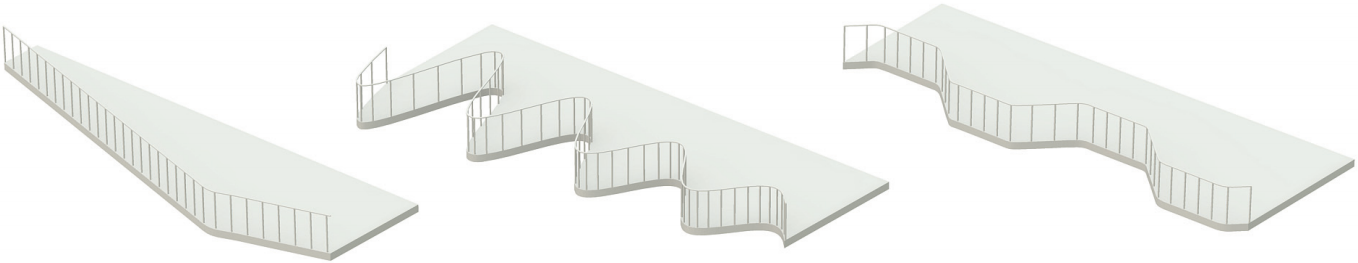
\includegraphics[width=\textwidth]{fig/balcony-variants}
  \caption[Different building balconies generated by different functions]{
    Three different balconies generated by different functions provided as
    arguments to the function that creates the building.  Retrieved from
  \cite{Leitao:2014:IGDAGHOP}.}
  \label{fig:intro.ad.balconies}
\end{figure}
\end{comment}
